\documentclass[a4paper,11pt,UTF8]{article}
\usepackage{ctex}
\usepackage{amsmath,amsthm,amssymb,amsfonts}
\usepackage{amsmath}
\usepackage[a4paper]{geometry}
\usepackage{graphicx}
\usepackage{microtype}
\usepackage{siunitx}
\usepackage{booktabs}
\usepackage[colorlinks=false, pdfborder={0 0 0}]{hyperref}
\usepackage{cleveref}
\usepackage{esint} 
\usepackage{graphicx}
\usepackage{ragged2e}
\usepackage{pifont}
\usepackage{extarrows}
\usepackage{mathptmx}
\usepackage{float}
\usepackage{caption}
\captionsetup[figure]{name={Figure}}

\title{Microelectronics Circuit Analysis and Design Homework(9th)}
\author{Yuejin Xie \quad U202210333}
\date{Oct 14th, 2023}
\begin{document}
\maketitle
7.3 Consider the circuit in Figure P7.3. (a) Derive the expression for the voltage transfer function $T(s) = V_o(s)/V_i (s)$.(b) What is the time constant associated with this circuit? (c) Find the corner frequency. (d) Sketch the Bode magnitude plot of the voltage transfer function.
\begin{figure}[H]
	\centering
	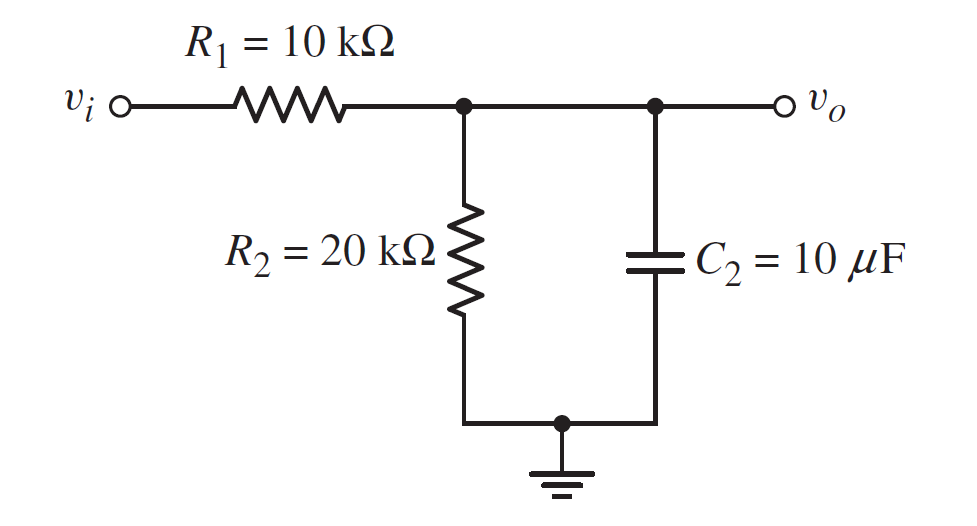
\includegraphics[scale=0.3]{MD7.3}
	\caption{Problem 7.3}
\end{figure}
Solution:

(a)Because of "KVL", we have equation:
$$
	\frac{V_o}{R_2||\displaystyle\frac1{sC_2}}R_1+V_o=V_i\\ \Rightarrow T(s)=\frac{V_o(s)}{V_i(s)}=\frac{R_{2}\left\|\displaystyle\frac{1}{sC_{2}}\right.}{R_{2}\left\|\displaystyle\frac{1}{sC_{2}}+R_{1}\right.}=\frac{R_{2}}{R_{1}+R_{2}+sR_{1}R_{2}C_{2}}
$$

(b)$\tau=(R_1||R_2)C_2=66.7\mathrm{ms}$

(c)$\displaystyle f=\frac{1}{2\pi\tau}=2.39\mathrm{Hz}$

(d)The Bode Plot is as follow(Use Python):
\begin{figure}[H]
	\centering
	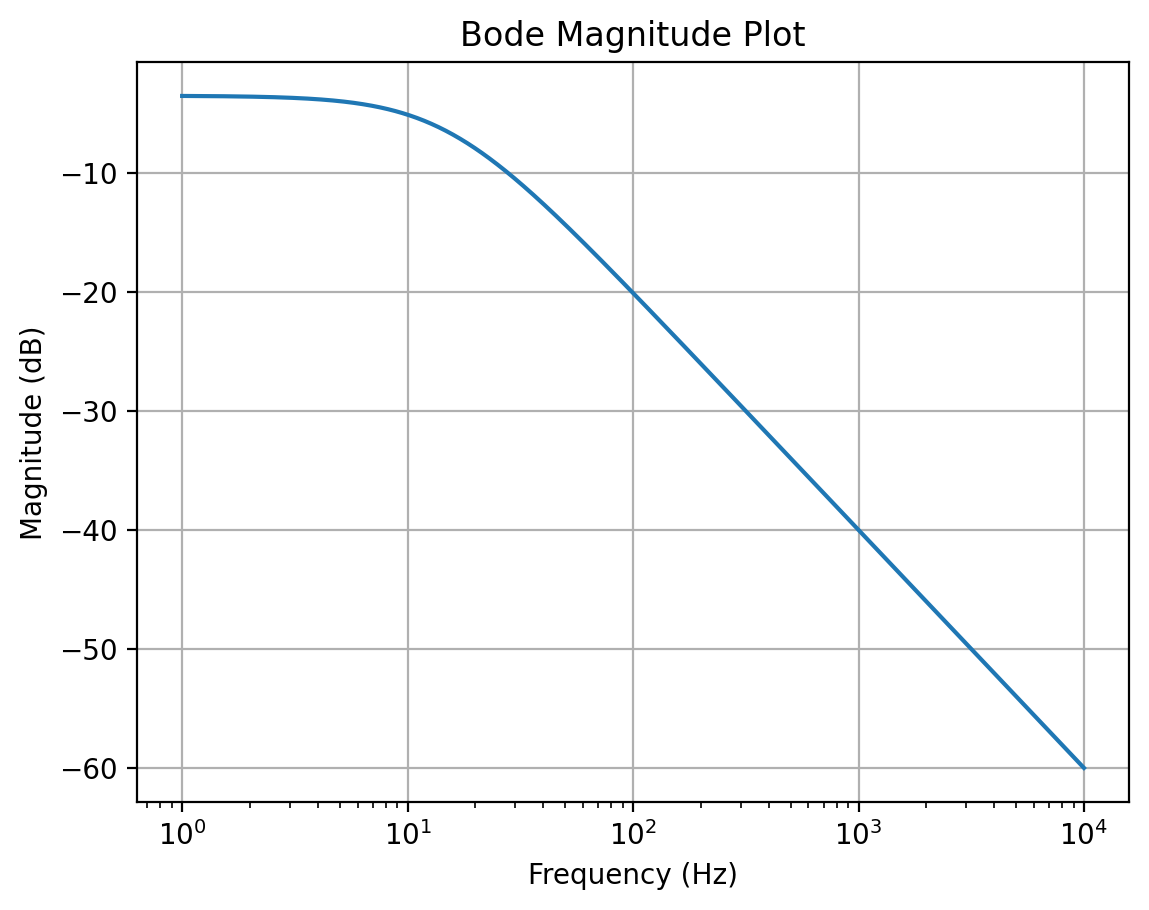
\includegraphics[scale=0.7]{MD7.3_1}
	\caption{7.3 Bode Plot}
\end{figure}
7.12 For the circuit shown in Figure P7.12, the parameters are $R_1 = 10 \mathrm{k\Omega},
R_2 = 10 \mathrm{k\Omega}, R_3 = 40 \mathrm{k\Omega}$, and $C = 10\mathrm{\mu F}$. (a) What is the value of the voltage
transfer function $V_o/V_i$ at very low frequencies? (b) Determine the value of the voltage transfer function at very high frequencies. (c) Derive the expression for the voltage transfer function $T (s) = V_o(s)/V_i(s)$. Put the expression in the form$ T(s) = K(1 + s\tau_A)/(1 + s\tau_B)$. What are the values
of $K, \tau_A,$ and $\tau_B$.
\begin{figure}[H]
	\centering
	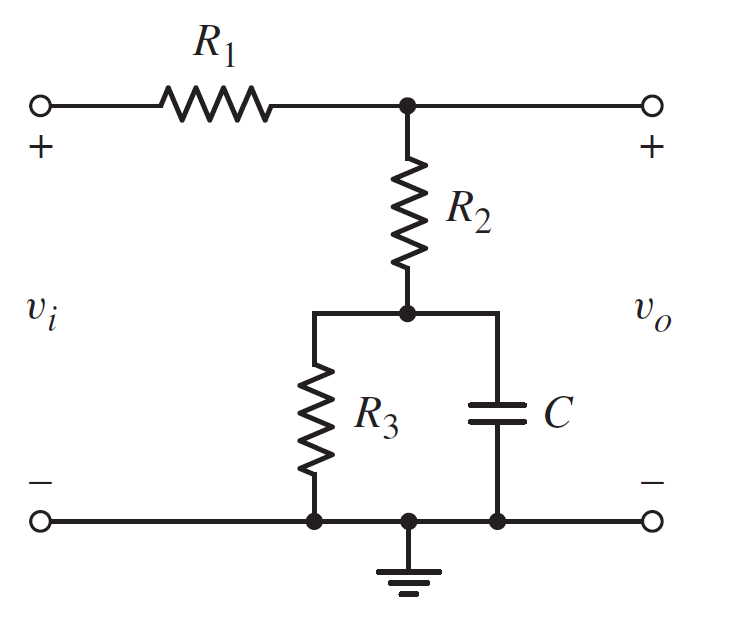
\includegraphics[scale=0.25]{MD7.12}
	\caption{Problem 7.12}
\end{figure}
Solution:

(a)In this case, the capacitor can be regarded as open, so the conclusion is obvious:
$$
	\frac{V_o}{V_i}=\frac{R_2+R_3}{R_1+R_2+R_3}=0.833
$$

(b)In this case, the capacitor can be regarded as shorted, so the conclusion is obvious:
$$
\frac{V_o}{V_i}=\frac{R_2}{R_1+R_2}=0.5
$$

(c)Because of voltage relationship, we have:
$$
	T(s)=\frac{R_2+R_3\left|\left|\displaystyle\frac1{sC}\right.\right.}{1+R_2+R_3\left|\left|\displaystyle\frac1{sC}\right.\right.}=\frac{R_{2}+R_{3}+sR_{2}R_{3}C}{R_{1}+R_{2}+R_{3}+s\bigl(R_{1}+R_{2}\bigr)R_{3}C}
$$

(d)We can easily get the answer by the conclusion of (c):
$$
	T(s)=\frac{R_{2}+R_{3}+sR_{2}R_{3}C}{R_{1}+R_{2}+R_{3}+s\bigl(R_{1}+R_{2}\bigr)R_{3}C}=\left(\frac{R_2+R_3}{R_1+R_2+R_3}\right)\cdot\frac{1+s\Big(R_2\Big\Vert R_3\Big)C}{1+s\Big(\Big(R_1+R_2\Big)\Big\Vert R_3\Big)C}
$$

$\therefore\displaystyle K=\frac{R_2+R_3}{R_1+R_2+R_3}=0.833, \tau_A=\Big(R_2\Big\Vert R_3\Big)C=80\mathrm{ms},\tau_B=\Big(\Big(R_1+R_2\Big)\Big\Vert R_3\Big)C=133.3\mathrm{ms}$

7.17 For the common-emitter circuit in Figure P7.17, the transistor parameters are: $\beta = 100, V_{BE(on)} = 0.7 $V, and $V_A =\infty$. (a) Calculate the lower corner frequency. (b) Determine the midband voltage gain. (c) Sketch the Bode plot of the voltage gain magnitude.
\begin{figure}[H]
	\centering
	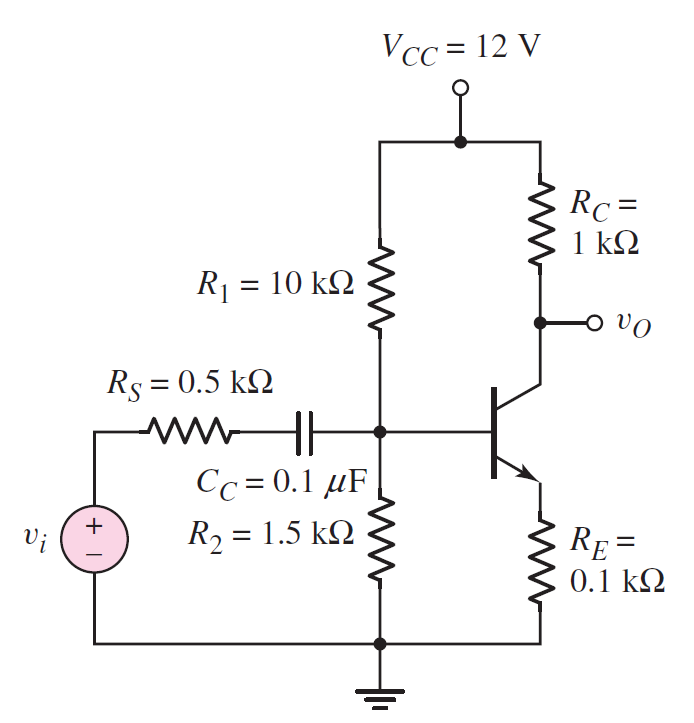
\includegraphics[scale=0.3]{MD7.17}
	\caption{Problem 7.17}
\end{figure}
Solution:

(a)We first find Q-point: $V_{TH}=\frac{R_2}{R_1+R_2}V_{CC}=1.565\mathrm{V},R_{TH}=R_1\left|\left|
\right.\right.R_2=1.304\mathrm{k\Omega}$. So KVL equation:
$$
	I_{BQ}R_{TH}+V_{BE(ON)}+(\beta+1)I_{BQ}R_E=V_{TH}\Rightarrow I_{BQ}=0.0759\mathrm{mA}
$$

$\displaystyle\therefore I_{CQ}=7.585\mathrm{mA},r_\pi=\frac{\beta V_T}{I_{CQ}}=0.343\mathrm{k\Omega}$

$\therefore R_{Si}=R_S=0.5\mathrm{k\Omega},R_{ib}=(R_{1}\left|\left|R_2\right.\right.)||(r_\pi+(\beta+1)R_E)=1.159\mathrm{k\Omega}\Rightarrow\tau=(R_{Si}+R_{ib})C=0.1659 \mathrm{ms}$

$\displaystyle\therefore f=\frac{1}{2\pi\tau}=959\mathrm{Hz}$

(b)
$$
	A_v=\frac{-g_m\left(\displaystyle\frac{(R_1\Vert R_2)\Vert (r_\pi+(\beta+1)R_E)}{(R_1\Vert R_2)\Vert (r_\pi+(\beta+1)R_E)+R_S}v_i\cdot \frac{r_\pi}{r_\pi+(\beta+1)R_E}\right)R_C}{v_i}=6.69
$$

(c)
\begin{figure}[H]
	\centering
	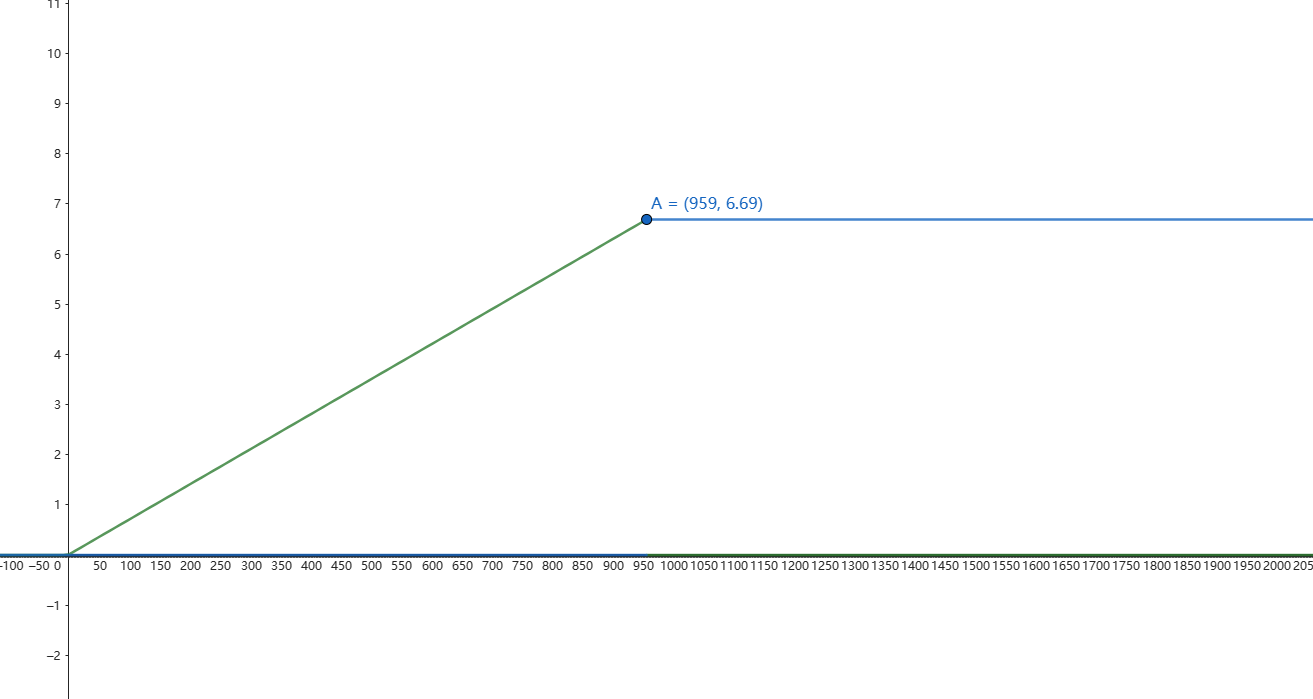
\includegraphics[scale=0.3]{MD7.17_1}
	\caption{7.17Bode plot}
\end{figure}
7.26 The parameters of the transistor in the circuit in Figure P7.26 are $K_p =1 \mathrm{mA/V^2}, V_{TP} = -1.5\mathrm{V},$ and $\lambda=0$. (a) Determine the quiescent and small-signal parameters of the transistor. (b) Find the time constants associated with $C_{C1}$ and $C_{C2}$. (c) Is there a dominant pole frequency? Estimate the -3 dB frequency.
\begin{figure}[H]
	\centering
	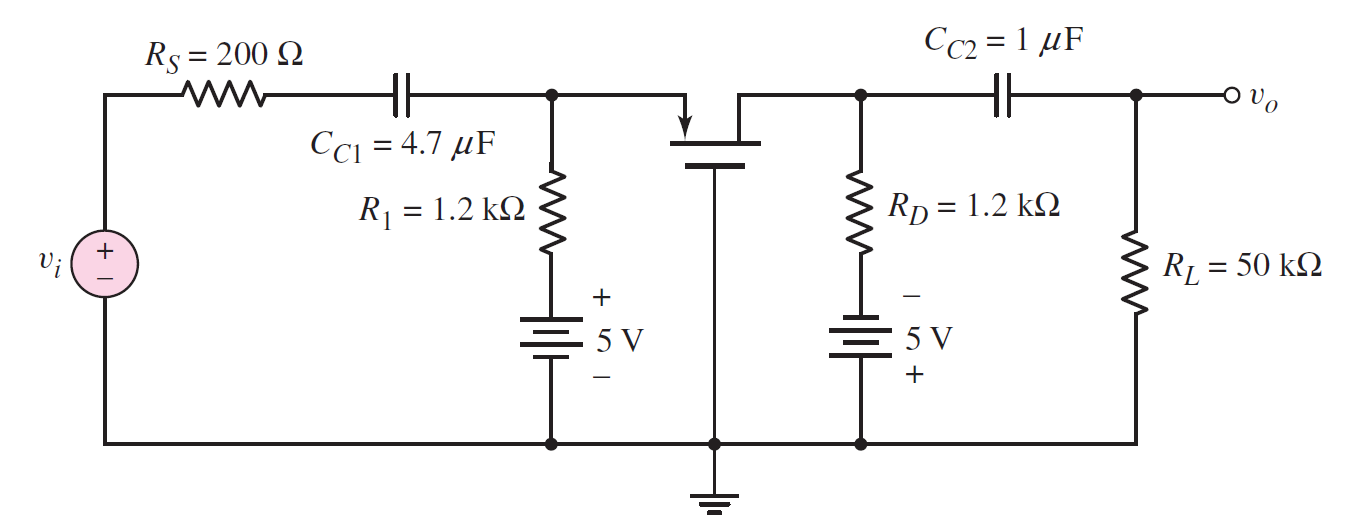
\includegraphics[scale=0.3]{MD7.26}
	\caption{Problem 7.26}
\end{figure}
Solution:

(a)We assume the MOS work in saturation region:
$$\frac{5-V_{SG}}{R_{1}}=K_{P}\left(V_{SG}+V_{TP}\right)^{2}\Rightarrow V_{SG}=2.84\mathrm{V}\Rightarrow I_{DQ}=1.8mA$$ 

$\therefore V_{SDQ}=10-1.8(1.2+1.2)\Rightarrow V_{SDQ}=5.68\mathrm{V} 
,g_{m}=2\sqrt{K_{P}I_{DQ}}=2.683\mathrm{mA/V}$ 

(b)$\displaystyle R_{Si}=\frac{1}{g_{m}}=\frac{1}{2.68}=0.3727\mathrm{k\Omega},R_{i}=1.2\parallel R_{Si}=0.284\mathrm{k\Omega}$

$C_{C1},\tau_{s1}=\left(284+200\right)\left(4.7\times10^{-6}\right)=2.27\mathrm{ms}$

$C_{C2},\tau_{s2}=\left(1.2x10^{3}+50\times10^{3}\right)\left(10^{-6}\right)=51.2\mathrm{ms}$  

(c)$C_{C2}$ dominates, $\displaystyle f_{3-dB}=\frac{1}{2\pi\tau_{s2}}=\frac{1}{2\pi\left(51.2\times10^{-3}\right)}=3.1\mathrm{Hz}$
\end{document}